\documentclass[tikz,border=12pt]{standalone}
\usepackage[T1]{fontenc}
\usepackage{mathpazo}
\usepackage{amsmath,amssymb}
\usetikzlibrary{arrows.meta, positioning, calc, fit, patterns, decorations.pathreplacing, 3d}

\definecolor{stblue}{HTML}{7B97AD}
\definecolor{rwgold}{HTML}{B8995E}
\definecolor{sage}{HTML}{7A9A7E}
\definecolor{dkbrown}{HTML}{3D3530}
\definecolor{wmgray}{HTML}{7B7067}
\definecolor{cream}{HTML}{F9F6F0}
\definecolor{border}{HTML}{D4C9B8}
\definecolor{terracotta}{HTML}{C47A6A}
\definecolor{lavender}{HTML}{907EA0}

\begin{document}
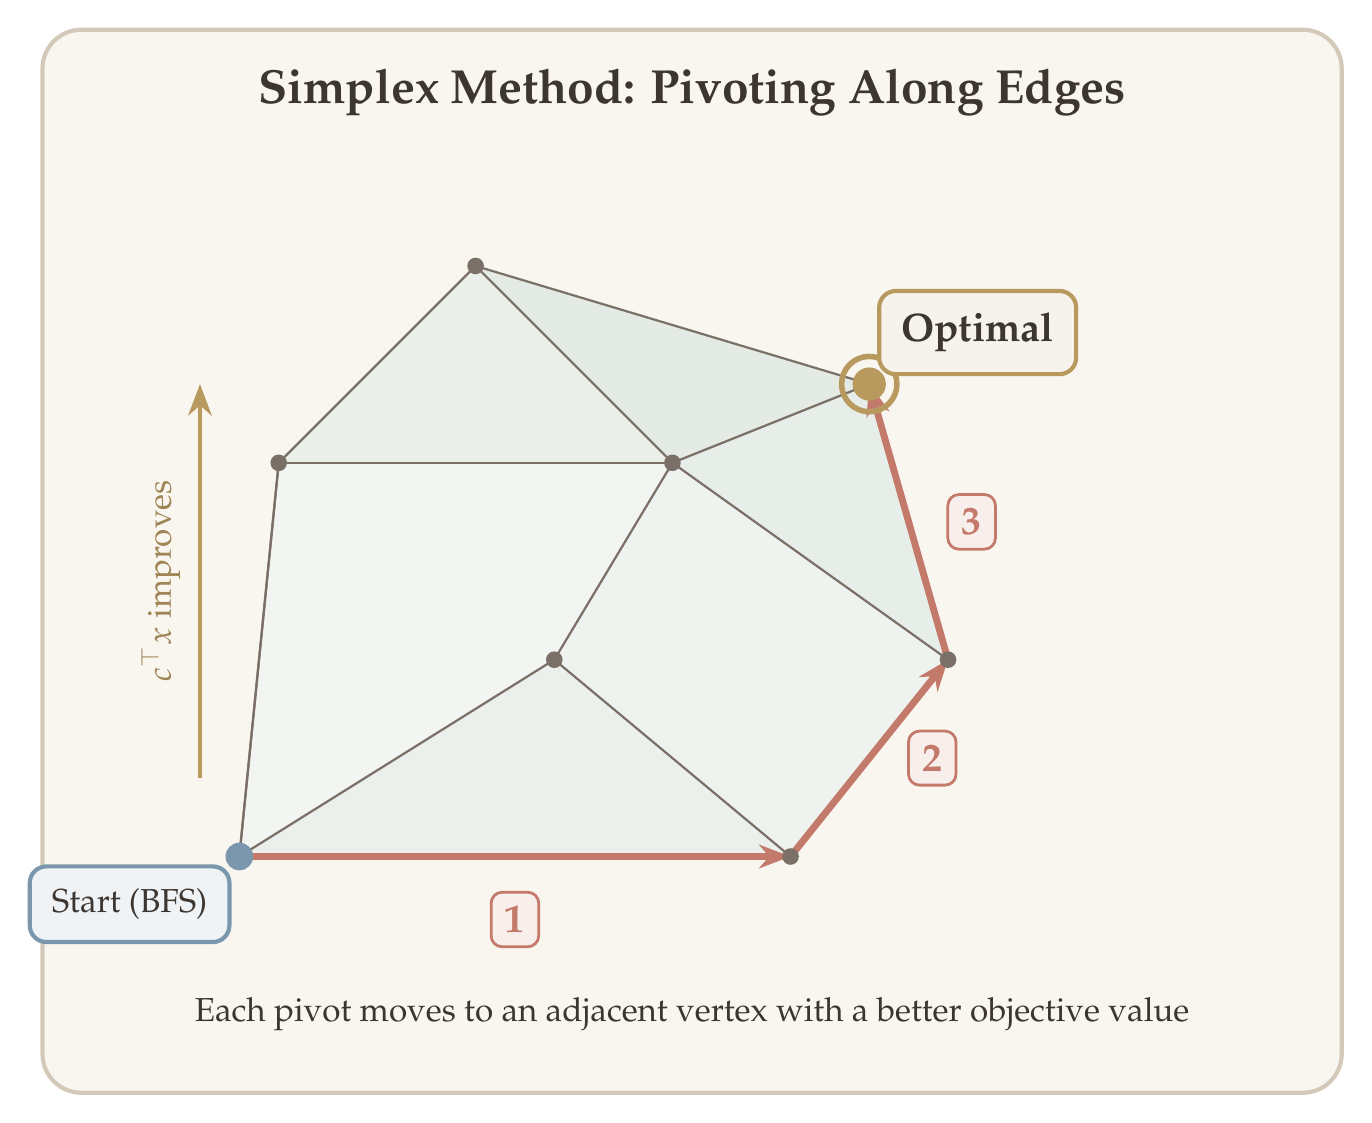
\begin{tikzpicture}[>={Stealth[length=4mm, width=3mm]}, line width=1.5pt]

% Background
\fill[cream, rounded corners=14pt] (-1.5,-2.5) rectangle (15,11);
\draw[border, line width=1.5pt, rounded corners=14pt] (-1.5,-2.5) rectangle (15,11);

% Title
\node[font=\LARGE\bfseries, text=dkbrown] at (6.75,10.2) {Simplex Method: Pivoting Along Edges};

% 3D-looking polytope vertices (projected)
\coordinate (A) at (1, 0.5);
\coordinate (B) at (8, 0.5);
\coordinate (C) at (10, 3);
\coordinate (D) at (9, 6.5);
\coordinate (E) at (4, 8);
\coordinate (F) at (1.5, 5.5);
\coordinate (G) at (5, 3);
\coordinate (H) at (6.5, 5.5);

% Back faces (lighter)
\fill[sage!8] (A) -- (G) -- (H) -- (F) -- cycle;
\fill[sage!8] (G) -- (B) -- (C) -- (H) -- cycle;

% Front faces
\fill[sage!15] (A) -- (B) -- (G) -- cycle;
\fill[sage!12] (B) -- (C) -- (H) -- (G) -- cycle;
\fill[sage!18] (C) -- (D) -- (H) -- cycle;
\fill[sage!20] (D) -- (E) -- (H) -- cycle;
\fill[sage!16] (E) -- (F) -- (H) -- cycle;
\fill[sage!10] (F) -- (A) -- (G) -- (H) -- cycle;

% Edges
\draw[wmgray, line width=0.8pt] (A) -- (B) -- (C) -- (D) -- (E) -- (F) -- cycle;
\draw[wmgray, line width=0.8pt] (A) -- (G) -- (B);
\draw[wmgray, line width=0.8pt] (G) -- (H);
\draw[wmgray, line width=0.8pt] (C) -- (H) -- (D);
\draw[wmgray, line width=0.8pt] (E) -- (H);
\draw[wmgray, line width=0.8pt] (F) -- (H);
\draw[wmgray, line width=0.8pt] (F) -- (A);

% Simplex path: A -> B -> C -> D (improving objective)
\draw[terracotta, line width=2.5pt, ->] (A) -- (B);
\draw[terracotta, line width=2.5pt, ->] (B) -- (C);
\draw[terracotta, line width=2.5pt, ->] (C) -- (D);

% Pivot numbers
\node[fill=terracotta!12, draw=terracotta, rounded corners=4pt, line width=1pt,
      font=\Large\bfseries, text=terracotta, inner sep=5pt]
  at ($(A)!0.5!(B) + (0,-0.8)$) {1};
\node[fill=terracotta!12, draw=terracotta, rounded corners=4pt, line width=1pt,
      font=\Large\bfseries, text=terracotta, inner sep=5pt]
  at ($(B)!0.5!(C) + (0.8,0)$) {2};
\node[fill=terracotta!12, draw=terracotta, rounded corners=4pt, line width=1pt,
      font=\Large\bfseries, text=terracotta, inner sep=5pt]
  at ($(C)!0.5!(D) + (0.8,0)$) {3};

% Starting vertex
\fill[stblue] (A) circle (5pt);
\node[fill=stblue!12, draw=stblue, rounded corners=6pt, line width=1.5pt,
      font=\large, text=dkbrown, inner sep=8pt, below left=4pt] at (A) {Start (BFS)};

% Optimal vertex
\fill[rwgold] (D) circle (6pt);
\draw[rwgold, line width=2pt] (D) circle (10pt);
\node[fill=rwgold!12, draw=rwgold, rounded corners=6pt, line width=1.5pt,
      font=\Large\bfseries, text=dkbrown, inner sep=8pt, above right=4pt] at (D) {Optimal};

% Other vertices
\fill[wmgray] (B) circle (3pt);
\fill[wmgray] (C) circle (3pt);
\fill[wmgray] (E) circle (3pt);
\fill[wmgray] (F) circle (3pt);
\fill[wmgray] (G) circle (3pt);
\fill[wmgray] (H) circle (3pt);

% Objective improvement annotation
\draw[->, rwgold, line width=1.5pt] (0.5,1.5) -- (0.5,6.5);
\node[font=\large, text=rwgold!80!dkbrown, rotate=90] at (0,4) {$c^\top x$ improves};

% Bottom note
\node[font=\large, text=dkbrown] at (6.75,-1.5)
  {Each pivot moves to an adjacent vertex with a better objective value};

\end{tikzpicture}
\end{document}
